%% LyX 2.3.7 created this file.  For more info, see http://www.lyx.org/.
%% Do not edit unless you really know what you are doing.
\documentclass[english]{article}
\usepackage[T1]{fontenc}
\usepackage[latin9]{inputenc}
\usepackage{float}
\usepackage{amssymb}
\usepackage{graphicx}

\makeatletter

%%%%%%%%%%%%%%%%%%%%%%%%%%%%%% LyX specific LaTeX commands.
\floatstyle{ruled}
\newfloat{algorithm}{tbp}{loa}
\providecommand{\algorithmname}{Algorithm}
\floatname{algorithm}{\protect\algorithmname}

\makeatother

\usepackage{babel}
\begin{document}
\title{Optimisation Algorithms for Machine Learning}
\title{Week 6 Assignment}
\author{Neimhin Robinson Gunning, 16321701}
\date{28th March 2024}

\maketitle
\textbf{(a) (i) Implementing mini-batch Stochastic Gradient Descent}

Our global loss function is
\[
f_{T}(x)=\sum_{w\in T}\frac{loss(x,w)}{\#W}
\]
which is just the average of $loss(w,x)$ ranging over the entire
dataset, $T$. We can also calculate an approximation of the loss
using a subset (minibatch) of $T$.
\[
f_{N}(x)=\sum_{w\in N}\frac{loss(x,w)}{\#N}
\]
This is implemented on line 17 of Algorithm~\ref{alg:minibatch-sgd}.
We can also approximate the gradient w.r.t. to the minibatch rather
than the full training dataset.

To generate mini-batches we first shuffle the rows data set and then
take successive slices with $n$ rows, where $n$ is the mini-batch
size. The first mini-batch consists of the 1st to the $n$th data
items, the second consists of the $(n+1)th$ to the $(n+n)th$, etc.
If we reach the end of the dataset before filling the minibatch we
shuffle the dataset and start again from index 1. This is implemented
on line 10 of Algorithm~\ref{alg:minibatch-sgd}.

The implementation of mini-batch SGD here relies on generating successive
$f_{N_{t}}$ and $\nabla f_{N_{t}}$, where $N_{t}$ is the mini-batch
for iteration $t$. This is implemented on line 40 of Algorithm~\ref{alg:minibatch-sgd}.

At each iteration the step size can be calculated with respect to
$f_{N_{t}}$ and $\nabla f_{N_{t}}$ using of the Polyak, RMSProp,
Heavy Ball, and Adam methods. Each of the step types are implemented
in \texttt{src/sgd.py} which is included in the appendix.

\begin{algorithm}
\begin{centering}
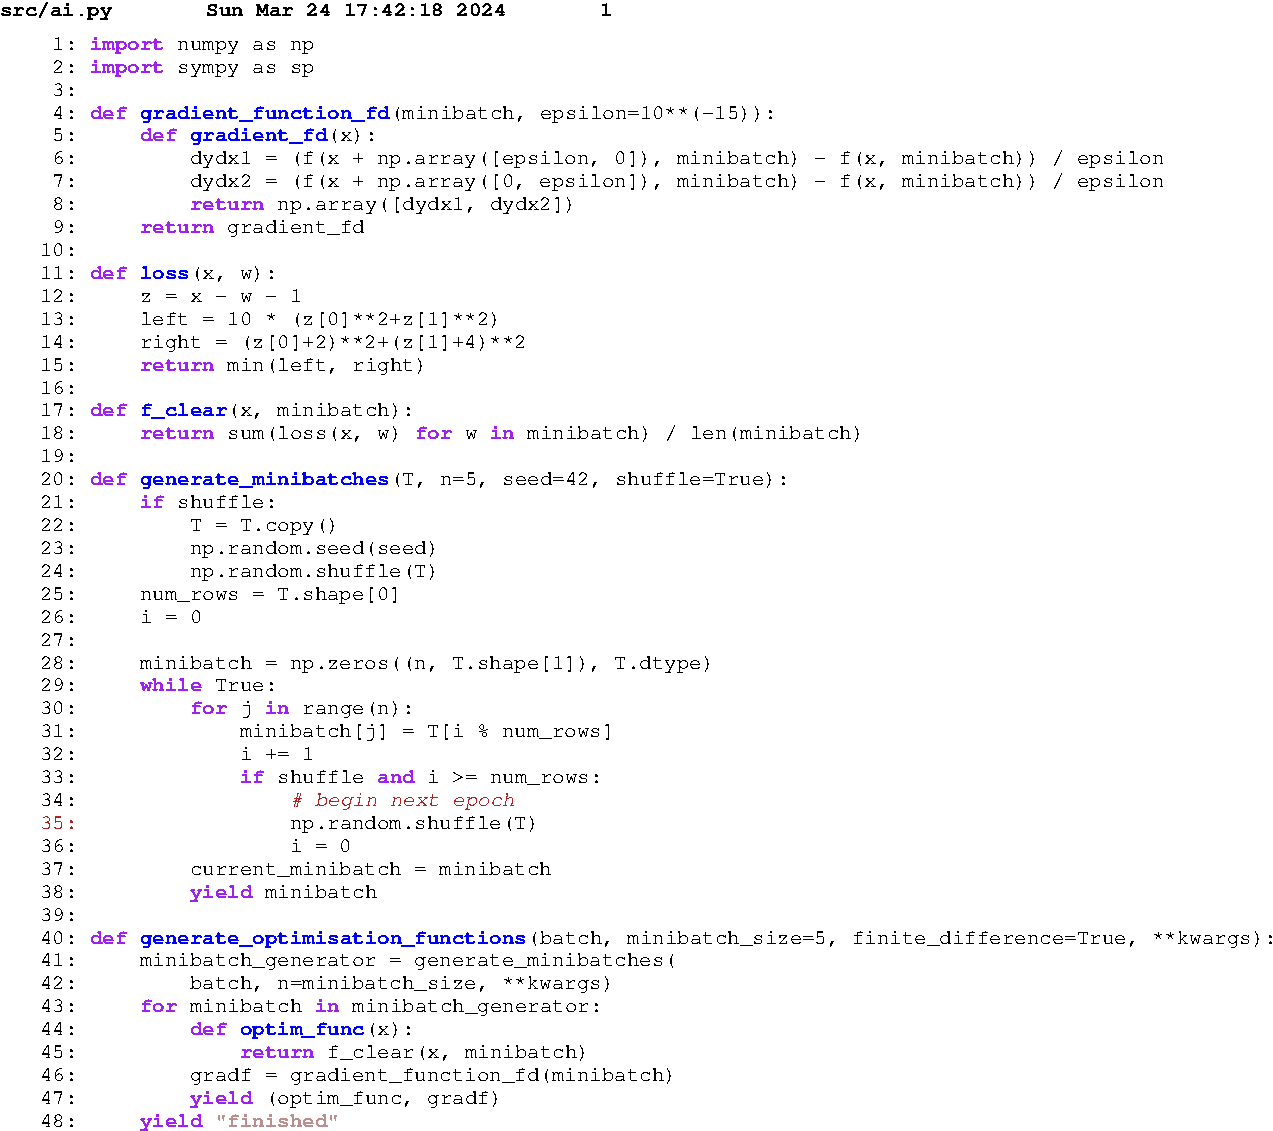
\includegraphics[width=0.9\textwidth]{fig/ai-code}
\par\end{centering}
\caption{\label{alg:minibatch-sgd}Generating mini-batches, $N$, and associated
$f_{N}$ and $\nabla f_{N}$.}
\end{algorithm}

\textbf{(a) (ii)}

We downloaded a pair of functions which are reproduced in Figure~\ref{fig:function-downloaded}.
On line 6 is a python definition of $f_{N}(x)$, where $N$ corresponds
to \texttt{minibatch}. We generate $T$ using lines 3 and 4 of Figure~\ref{fig:function-downloaded},
and use the same $T$ throughout the remainder of the discussion.
A wireframe and a contour plot of $f_{T}(X)$ is presented in Figure~\ref{fig:wireframe-and-contour},
showing $x\in[-5,5]^{2}$.

\begin{figure}
\begin{centering}
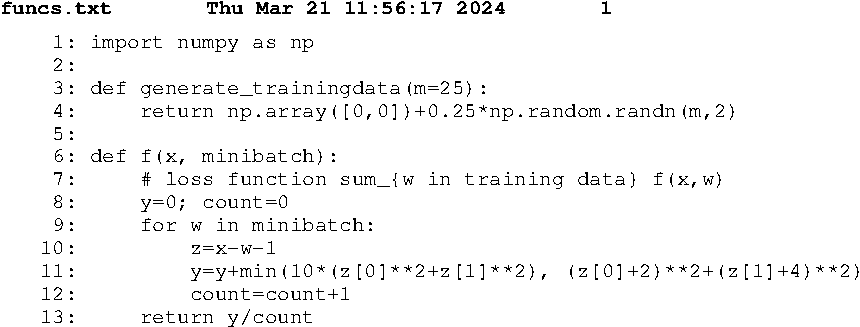
\includegraphics[width=0.8\textwidth]{funcs}
\par\end{centering}
\caption{\label{fig:function-downloaded}Functions downloaded for this assignment
from \url{https://www.scss.tcd.ie/Doug.Leith/CS7DS2/week6.php}.}
\end{figure}

\begin{figure}
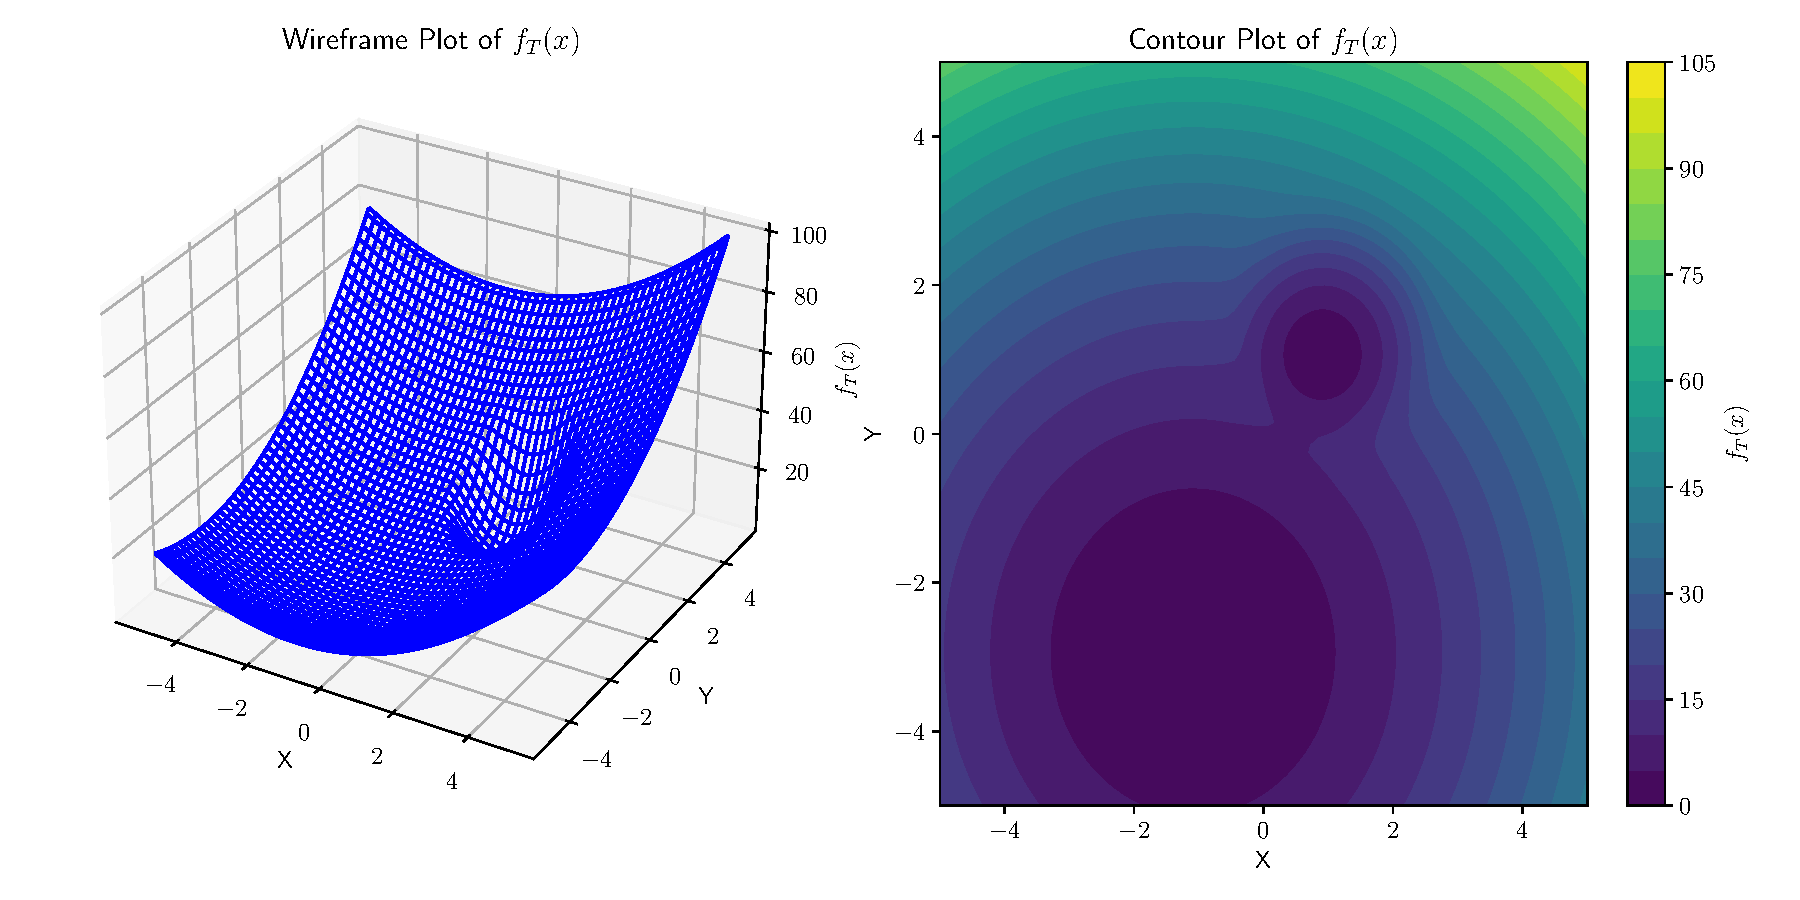
\includegraphics{fig/wire-contour}

\caption{\label{fig:wireframe-and-contour}Wireframe (left) and contour (right)
plots of $f_{T}(x)$ where $T$ is a `training set' generated by the
code in lines 3 and 4 of Figure~\ref{fig:function-downloaded}.}
\end{figure}

\textbf{(a) (iii) Gradient Calculation}

Implementations of both analytic calculation of gradients with sympy
and finite difference are provided in \texttt{src/week6.py}. Our
implementation of analytic calculation of gradients with sympy is
unfortunately dirt-slow, so in these experiments we use the finite
difference methods to estimate the mini-batch gradient according to
\[
\frac{df_{N}}{dx_{i}}\approx\frac{f_{N}([x_{1},\ldots,x_{i}+\epsilon,\ldots,x_{d}])-f_{N}(x)}{\epsilon}
\]
where we set $\epsilon=10^{-15}$ for the remainder of this discussion.
We also look at only at an example with $d=2$, i.e. $x\in\mathbb{R}^{2}$
so the finite difference gradient function $\nabla f_{N}:\mathbb{R}^{2}\rightarrow\mathbb{R}$
is:
\[
\nabla f_{N}(x)=[\frac{f_{N}([x_{1}+\epsilon,x_{2}])-f_{N}(x)}{\epsilon},\frac{f_{N}([x_{1},x_{2}+\epsilon])-f_{N}(x)}{\epsilon}]
\]
This works by calculating the slope after a small perterbation to
$x_{1}$ and then again a small perterbation to $x_{2}$. The code
implementation of this is on line 4 in Algorithm~\ref{alg:minibatch-sgd}.

\textbf{(b) (i) Gradient Descent with constant step-size}

Several runs of gradient descent with various constant step-sizes,
$\alpha$, are presented in Figure~\ref{fig:gd-constant}. The starting
estimate is $x=[3,3]$. The function $f_{T}(x)$ has a local minimum
at about $x=[1,1]$, but the global minimum is somewhere around $x=[-1,-3]$.
A careless choice of $\alpha$ results in converging to the suboptimal
local minimum, e.g. $\alpha=0.01$. Either of $\alpha=0.72$ or $\alpha=0.5$
are reasonabl choices. For $\alpha>0.72$ we see divergence. The lowest
value of $F_{T}(x)$ for the $\alpha=0.72$ run is marginally better
than for the $\alpha=0.5$ run, however, the $\alpha=0.5$ converges
marginally faster. For later experiments, where we are using Stochastic
Gradient Descent, the noise caused by mini-batches will mean that
we could diverge with lower values of $\alpha$, so from here on we
select $\alpha=0.5$ rather than $\alpha=0.72$ to mitigate the risk
of divergence.

\begin{figure}
\begin{centering}
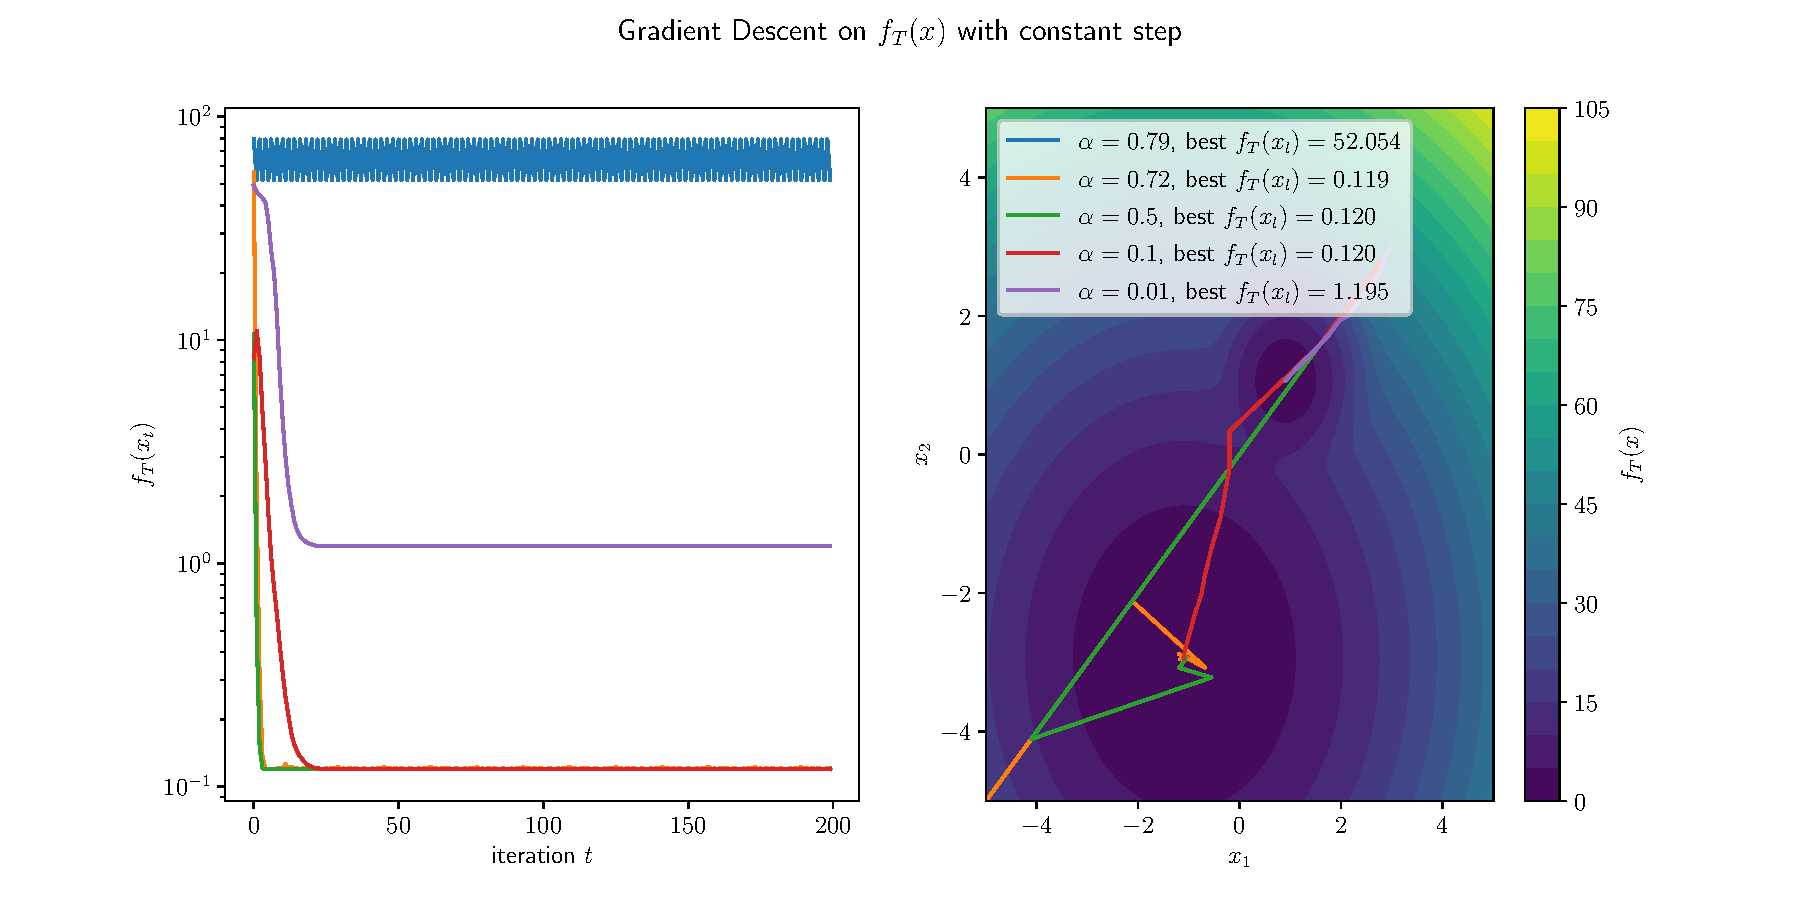
\includegraphics[width=1\textwidth]{fig/bi}
\par\end{centering}
\caption{\label{fig:gd-constant}Visualizations of gradient descent on $f_{T}(x)$
using a constant step size $\alpha$. On the left the function value
is plotted against the iteration number. On the write the successive
$x_{t}$s are plotted on a contour plot of $f_{T}(x)$.}
\end{figure}

\textbf{(b) (ii) Stochastic Gradient Descent with constant batch-size
and step-size}

4 runs of Stochastic Gradient Descent with constant batch-size, $n=5$,
and constant step size $\alpha=0.5$ are presented in Figure~\ref{fig:bii-sgd-constant}.
Each run is different due to the randomness introduced by sampling
the batches. The first step for three of the runs is broadly in the
direction of the global minimum, but the first run, run 0, has a first
step which is about $70^{\circ}$ off. Nonetheless, this run's overall
trajectory is very similar to the those of the others. Even when a
run achieves an $x_{t}$ that minimizes $f_{T}(.)$ the run continues
to `explore' a region due to the noise introduced by mini-batches,
i.e. the gradients are like a random variables drawn from $U(0,k)$.
However, the further the current estimate is from the a local minimum,
the more coherent are the gradients $\nabla f_{N_{t}}$, $\nabla f_{N_{t+1}}$,
etc., where $N_{t}$, $N_{t+1}$ etc. are different mini-batches.
This greater coherence at a distance is what allows the algorithm
converge to similar values on most runs. It is possible for the algorithm
to diverge with the same hyper parameters, $\alpha=0.5$ and mini-batch
size of 5, but that did occur for any of the 4 runs presented here.
The gradient descent runs reported above in \textbf{(b) (ii)} have
no randomness, so using $\alpha=0.5$ gives the same results every
time.

\begin{figure}
\begin{centering}
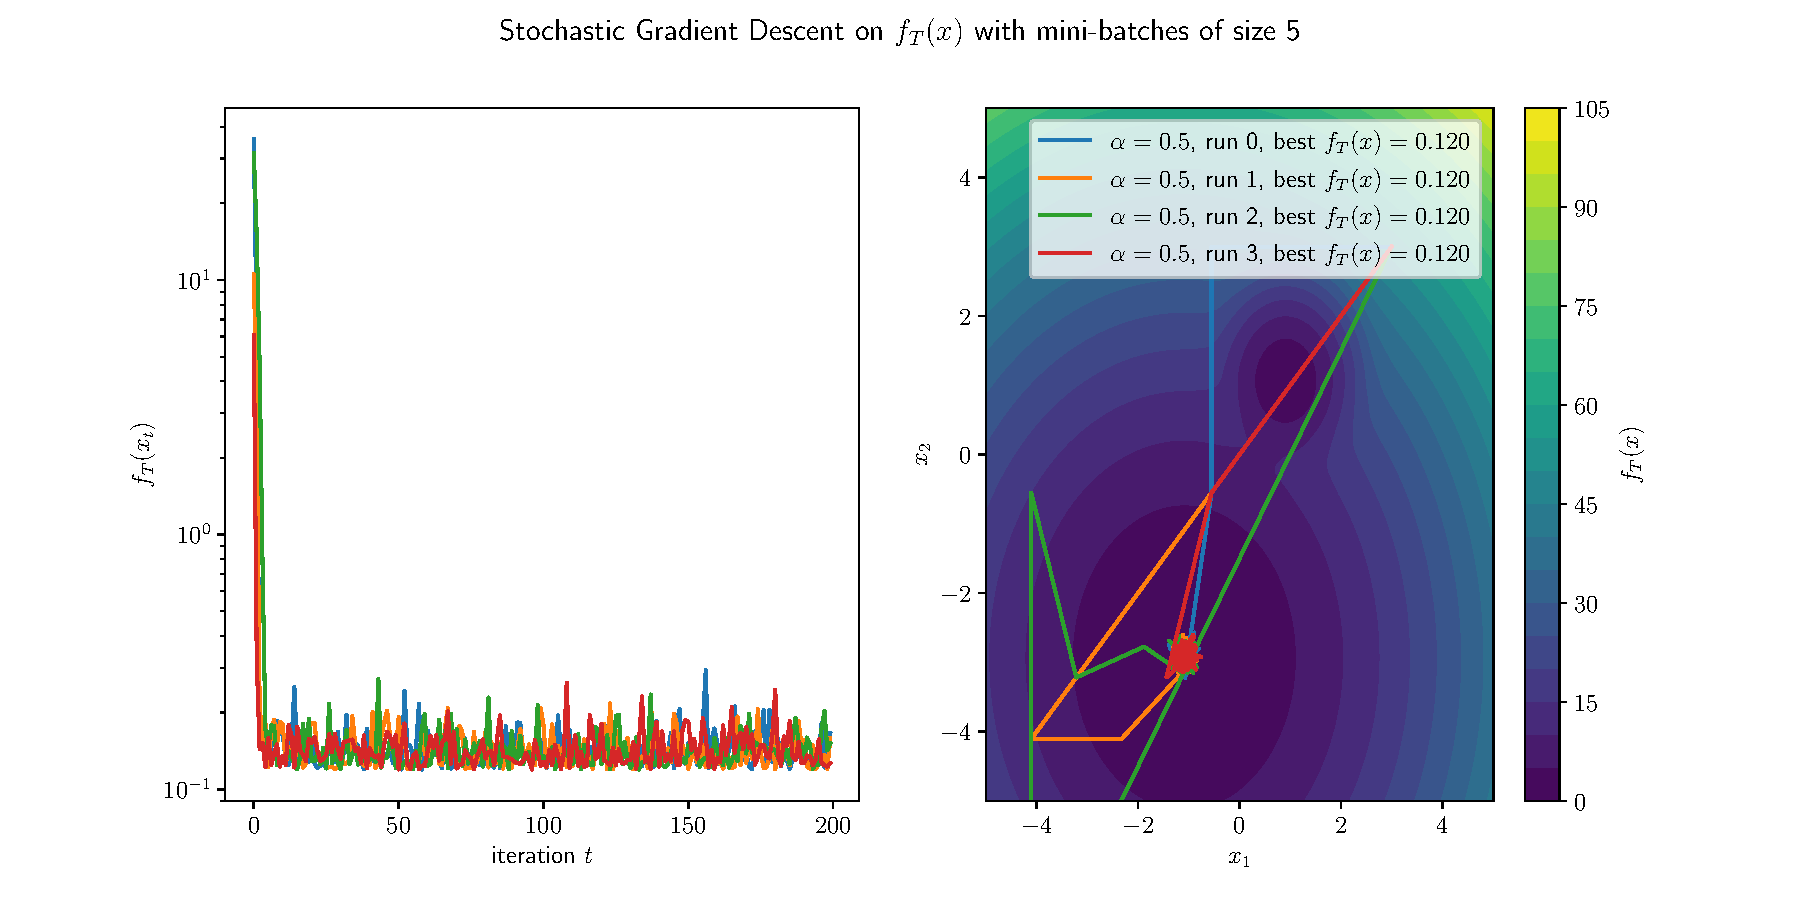
\includegraphics[width=1\textwidth]{fig/bii}
\par\end{centering}
\caption{\label{fig:bii-sgd-constant}Visualizations of gradient descent on
$f_{N_{t}}(x)$ using a constant step size $\alpha$. $N_{t}$ is
drawn from $T$ by first shuffling $T$ and slicing $T$ into batches
of size 5. On the left the function value is plotted against the iteration
number. On the write the successive $x_{t}$s are plotted on a contour
plot of $f_{T}(x)$.}
\end{figure}

\textbf{(b) (iii) Effect of Varying batch-size}

We look at a broad range of batch sizes in Figure~\ref{fig:biii-vary-batch-size},
from 1 up to $25=\#T$. In each case the SGD eventually hits a floor
and then jumps around near that floor. The distance of jumps it takes
from that floor is directly related to the batch-size. With lower
batch-size it takes larger jumps, i.e. there is greater noise for
lower batch. When $n=25=\#T$, there is no noise, we calculate gradient
with respect to the full set $T$ each time. There is no particular
relationship between $n$ and the final value of $f_{T}(x)$, however
there may be a relationship between $n$ and the \textbf{best} (i.e.
lowest) value of $f_{T}(x)$ observed for the run.

\begin{figure}
\begin{centering}
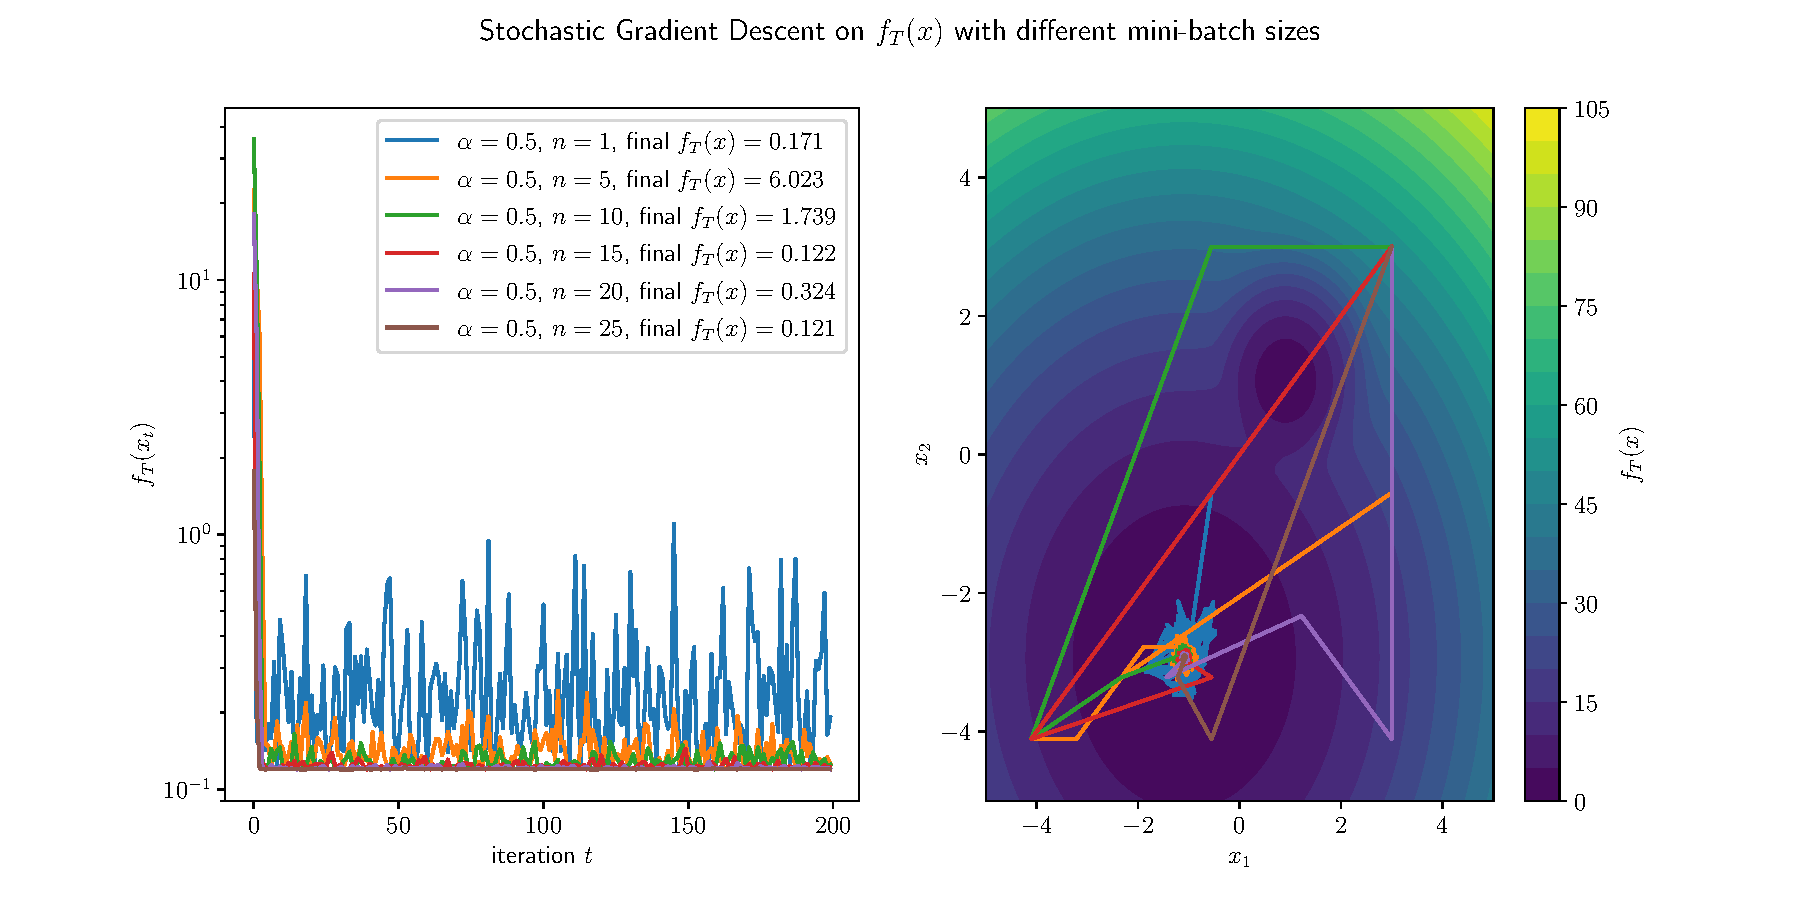
\includegraphics[width=1\textwidth]{fig/biii}
\par\end{centering}
\caption{\label{fig:biii-vary-batch-size}Visualizations of stochastic gradient
descent on $f_{T}(x)$ with various batch-sizes.}
\end{figure}

In Figure~\ref{fig:biii2-vary-batch-size} we again vary $n$ but
in a narrower range (1-15) and for fewer iterations (15). There is
no particular relationship between $n$ and the speed with which $f_{T}(x)$
initially descends. In this experiment $f_{T}(x)$ is calculated at
every iteration, which may be prohibitively expensive for optimisation
problems with much larger datasets, so it is not necessarily practical
to keep track of the best $f_{T}(x)$, but the data in Figure~\ref{fig:biii2-vary-batch-size}
do seem to indicate that a higher $n$ increases the chances of a
lower best $f_{T}(x)$. A reason for this might be that around the
noise floor, using higher $n$ means not jumping as far from the optimal
region, and taking smaller jumps because the noise is less significant.
This increases the chances of landing at a globally optimal value
for $x$, because the interval effectively being searched is smaller.

\begin{figure}
\begin{centering}
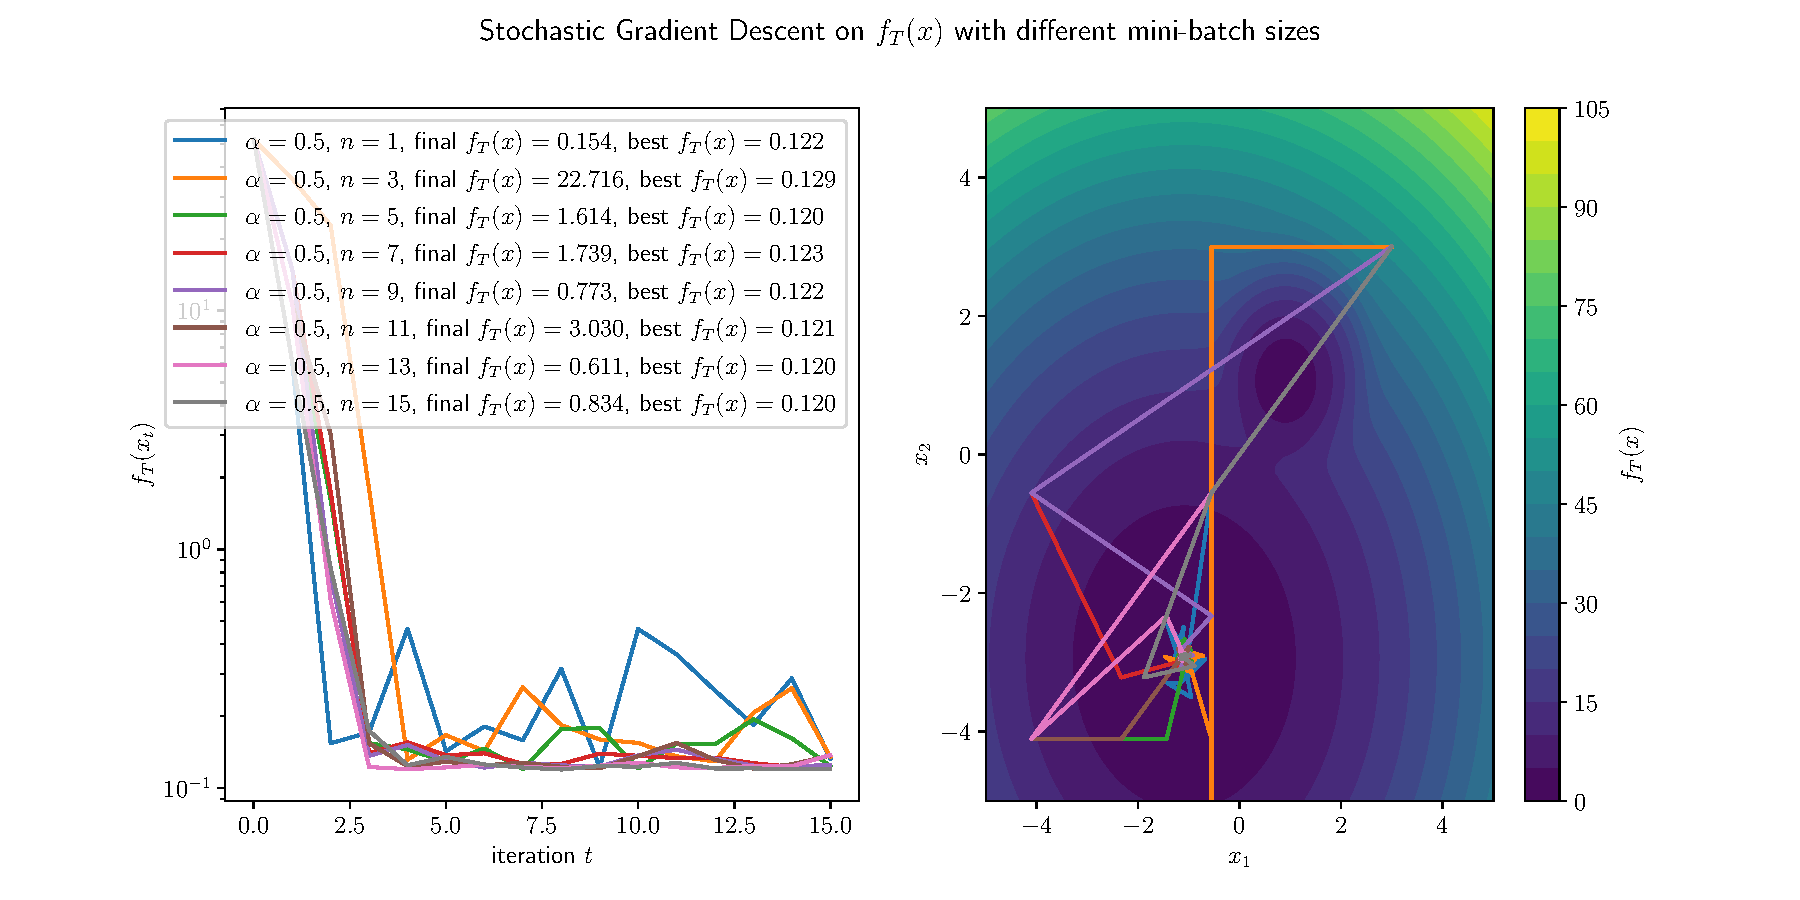
\includegraphics[width=1\textwidth]{fig/biii_2}
\par\end{centering}
\caption{\label{fig:biii2-vary-batch-size}Visualizations of stochastic gradient
descent on $f_{T}(x)$ with various batch-sizes and fixed $\alpha$.}
\end{figure}

\textbf{(b) (iv) SGD with various step-sizes}

In Figure~\ref{fig:biv} we present various runs of SGD, each with
the same batch-size $n=5$, but different step sizes $\alpha$. The
runs are set up with the same random seed such that the sequence of
batches, $N_{t},N_{t+1}$, is equivalent for each run, in order to
isolate the effect of changing $\alpha$. With $\alpha=0.001$ the
alg has similar behaviour to $\alpha=0.1$ except taking many more
iterations to follow the same trajectory. At $\alpha=0.01$ the alg
converges to the suboptimal local minimum. With $\alpha=1$ the alg
gets trapped for a time at a distance from the global minimum, but
eventually get very close the global minimum, and then hops out again
to fairly inaccurate estimates, diverging. The effect of the noise
from stochastic batch sampling is seemingly amplified by a larger
step size, such that for larger $\alpha$ we see a larger final search
radius after approaching the noise floor, and a greater chance of
diverging due to the noise, i.e. the chances of having a large unlucky
step in the wrong direction. Where the batch-size $n$ has a limited
range of values, $[0,\#T]$, we can vary $\alpha$ arbitrarily in
$\mathbb{R}^{+}$, and so if we want to tune just one hyperparameter
rather than two, e.g. due to compute cost, then it may beneficial
fix $n$ and vary $\alpha$.

By adjusting $\alpha$ we can achieve a noise level similar to the
effect of decreasing $n$ as we saw in section \textbf{(b) (iii) }above.
This noise can be beneficial as seen in the run with $\alpha=0.01$
in Figure~\ref{fig:biv}. For this run the alg initially gets stuck
in the suboptimal local minimum but eventually hops out and then converges
to the global minimum.

\begin{figure}
\begin{centering}
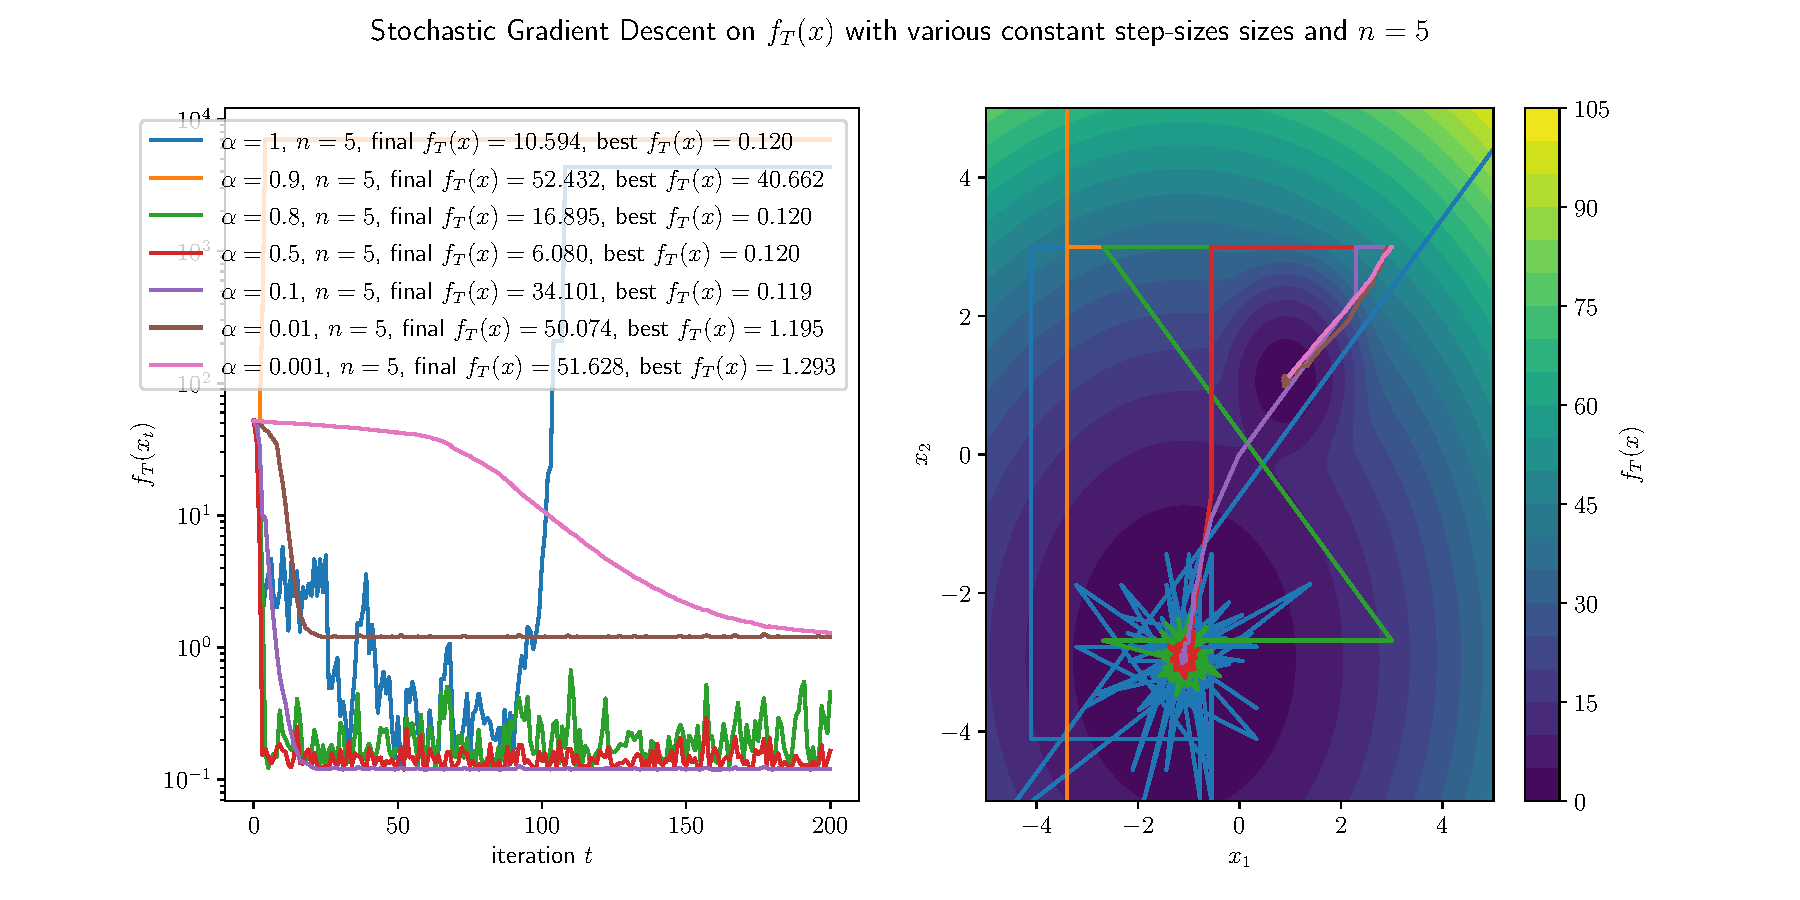
\includegraphics[width=1\textwidth]{fig/biv}
\par\end{centering}
\caption{\label{fig:biv}Visualizations of stochastic gradient descent on $f_{T}(x)$
with fixed batch-size $n=5$, and varioust constant step-sizes, $\alpha$.}
\end{figure}

\textbf{(c) (i) SGD with Polyak step}

Runs of SGD with Polyak step, $f^{*}=0.119$, and $n=1,3,5,7$ are
presented in Figure~\ref{fig:ci}. If there is a relationship between
$n$ and the behaviour of the alg, the relationship is not strong.
The experiment is run twice, with different random seeds, and there
is no consistency between the two experiments. With seed=58 we see
the alg converge to the suboptimal local minimum when $n=1$, but
with seed=59 the behaviour is different, it first explores the global
minimum and then `hops out' to the suboptimal local minimum. When
we increase $n$ to $7$ we see the alg first explore the suboptimal
local minimum and the `hop out' to the global minimum. From these
experiments there is no apparent stable relationship between $n$
and the alg's behaviour.

When we don't use SGD, i.e. when $n=25$, we see significantly smaller
steps once the alg has approached the global minimum, so choosing
$n<<\#T$ does significantly change the behaivour compared to $n=25$.

\begin{figure}
\begin{centering}
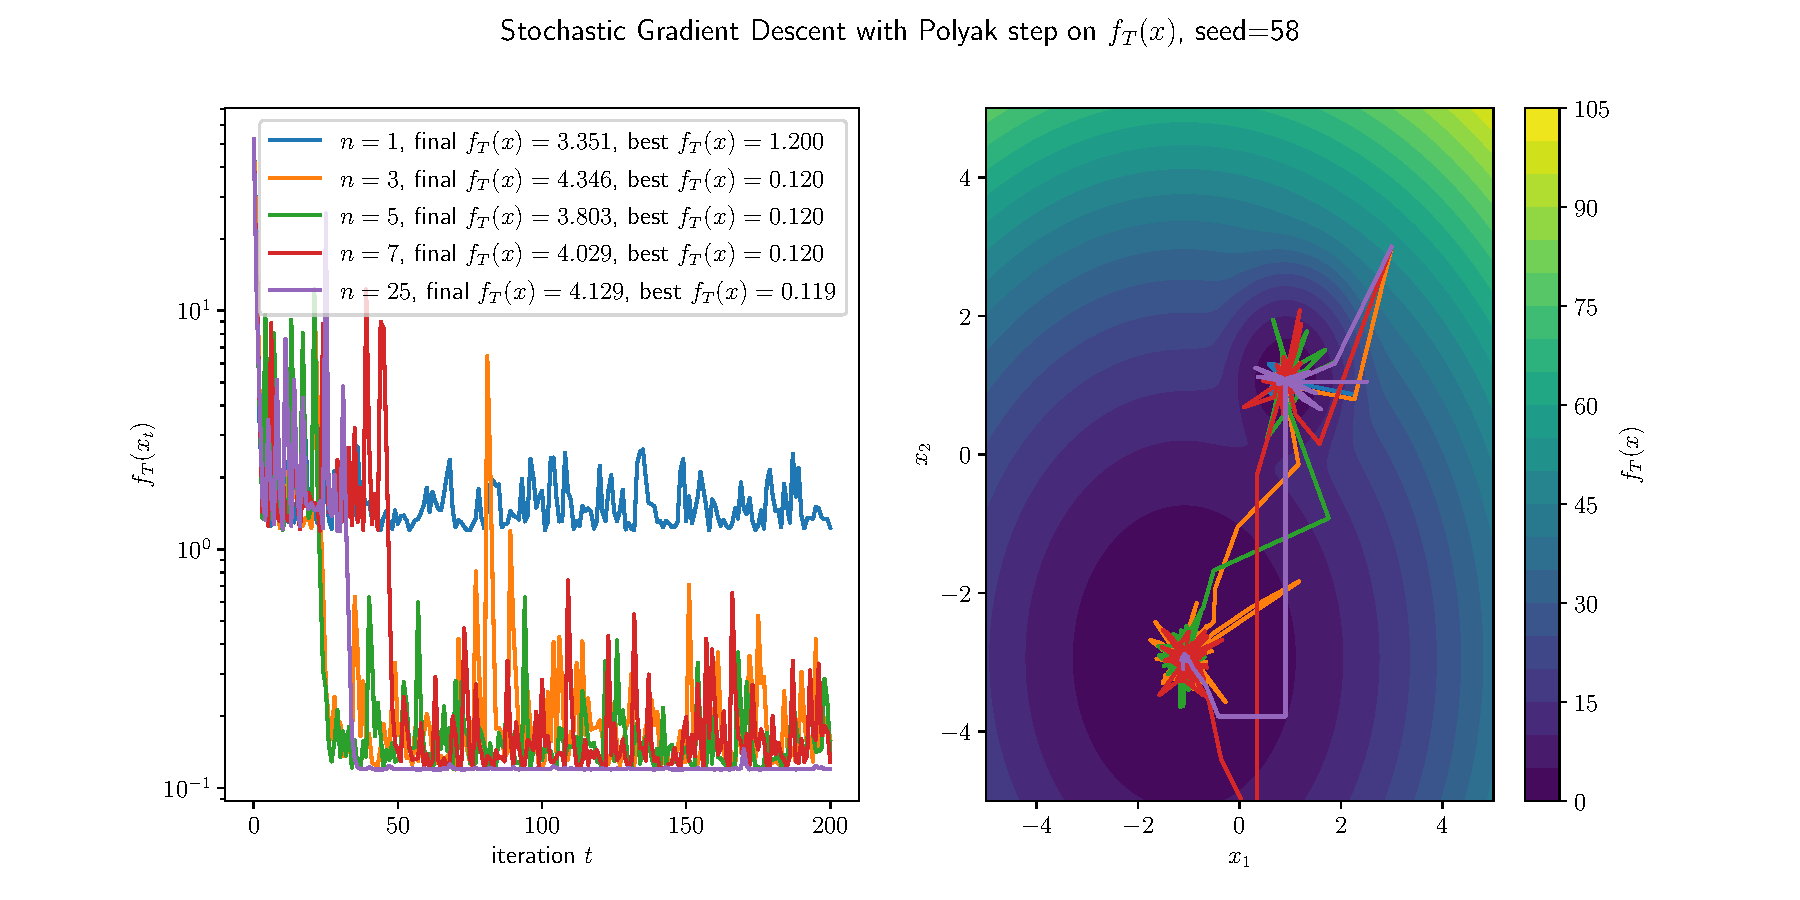
\includegraphics[width=1\textwidth]{fig/ci-58}
\par\end{centering}
\begin{centering}
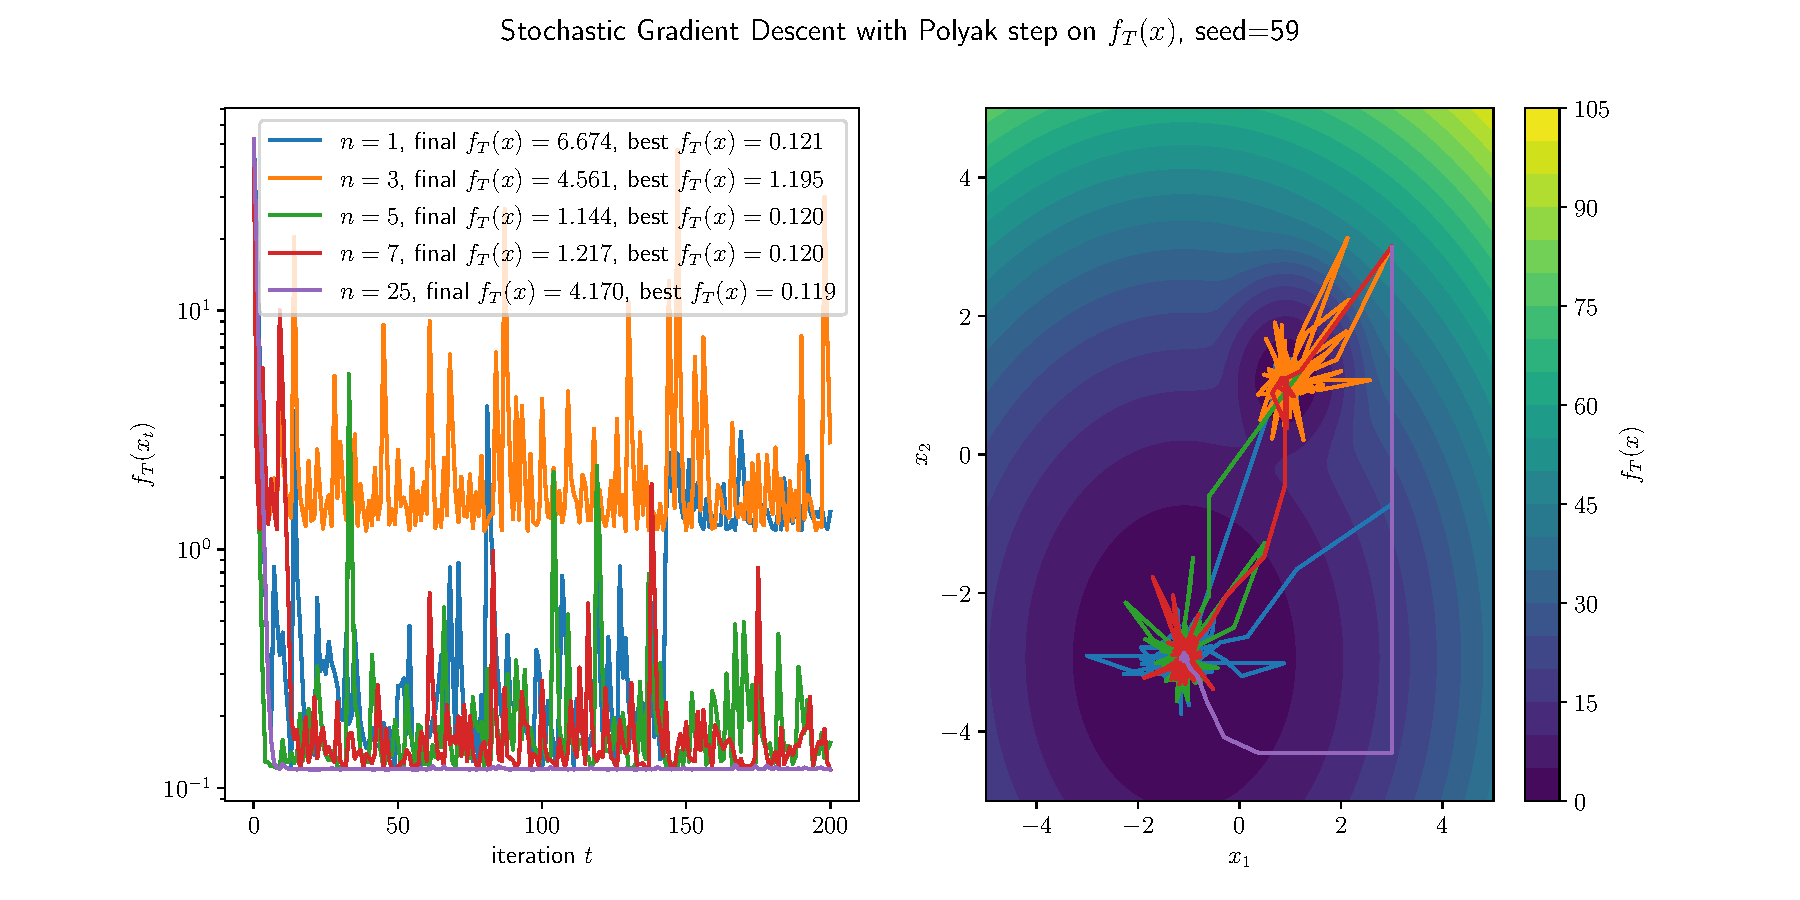
\includegraphics[width=1\textwidth]{fig/ci-59}
\par\end{centering}
\caption{\label{fig:ci}Visualizations of stochastic gradient descent on $f_{T}(x)$
with Polyak step and various $n$.}
\end{figure}

\end{document}
